
To judge the degradation of predictions of the algorithms with decreasing
information quality (detailed in Section \ref{sec:inforeduc2}), a plot for each
energy window list (auto, short, and long) is presented.  Figure \ref{fig:rxtr}
shows the balanced accuracy of reactor type classification for the previously
described \textit{x}-axis, where a score of $1$ is perfect prediction and a
score of $0$ is random classification. The error bars (which are not visible
past the marker size on the plots) reflect a 99\% confidence interval.  The
blue line that indicates an ideal performance is at 0.84 balanced accuracy,
which is based on the lowest performance of all three algorithms at 20\%
training set error for the 29 nuclide mass training set in Figure
\ref{fig:randerrA}.  The red line that indicates a baseline/minimum acceptable
performance is at a balanced accuracy score of 0.75, which is an arbitrary
choice. 

\begin{figure}[!htb]
  \centering
  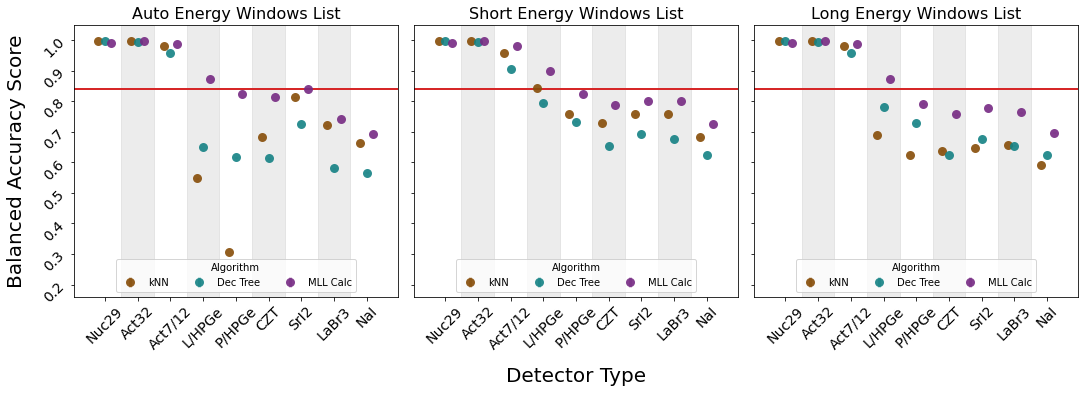
\includegraphics[width=\textwidth]{./chapters/exp2/detector_preds_wrt_enlist_BalAcc_rxtr.png}
  \caption{Prediction performance of reactor type as measured by balanced 
           accuracy with respect to decreasing detector energy resolution 
           for three types of processed gamma spectra.}
  \label{fig:rxtr}
\end{figure}

For the auto and short energy windows lists, the \textit{k}-nearest neighbors
performance is usually below \gls{MLL} calculations and above decision trees,
which is not expected. In Figure \ref{fig:randerrA}, the \textit{k}-nearest
neighbors line emerges with the lowest performance with decreasing information,
and it is interesting that this pattern did not emerge with the detectors'
performances. For the lab-based and portable \gls{HPGe}s, \textit{k}-nearest
neighbors has the worst performance for the auto and long lists, and
drastically so for the auto list cases. There are a few instances of
\textit{k}-nearest neighbors being above the red line: portable \gls{HPGe} for
the short list, \gls{SrI2} for the auto and short lists, and \gls{LaBr3} for
the short list. Also, the lab-based \gls{HPGe} exceeds the blue line.

For the short and long energy windows lists, decision trees only performs above
the red line for the lab-based \gls{HPGe} detector, and the remaining detectors
have a decision trees performance below the baseline; there is no detector for
which decision trees performs above the baseline on the auto list plot.
Decision trees almost consistently performs the worse for the last four
detectors.

For the short and long energy windows lists, \gls{MLL} is above the baseline
except for the \gls{NaI} detector.  For the auto list, only the last two
detectors (\gls{LaBr3} and \gls{NaI}) are below the red line.  The majority of
the data points for \gls{MLL} do not exceed the blue line, except for the
following cases: lab-based \gls{HPGe} for all three lists, and \gls{SrI2} for
the auto energy windows list.

Only the first three \textit{x}-axis categories exceed the blue line for all
three algorithms, which is expected for the various levels of full-knowledge
represented. The short energy windows list has the most data points above the
red line, and so can be declared to perform the best among the three lists for
reactor type prediction.  The slightly worse outcomes for the long energy
windows list are to be expected from the algorithms having to deal with a lot
of non-useable features, \todo{add this warning to i-reduc} especially for the
last four detectors.  The variable behavior of the auto energy windows list
would require further study, but the fact that the \gls{SrI2} detector
ouperforms all of the solid state detectors speaks to how an automatic peak
search should not be discarded as a method. This set of points outperforms even
the portable \gls{HPGe} on the short energy windows list.

As in Section \ref{sec:randerr}, the reactor type classification performance
discussion would not be complete without the added detail that confusion
matrices supply. First, the four "full knowledge" training sets are presented
in Figure \ref{fig:cm_nucs_acts}.  The 29 nuclide mass training set (top panel)
is repeated from the 1\% training set error case in Figure \ref{fig:cm_nuc29}.
For the 32 nuclide activity training set (second panel), the numbers are
approximately the same, but interestingly, they improve slightly for
\textit{k}-nearest neighbors and \gls{MLL} calculations.  A visible increase in
misclassification is clear with the 12 and 7 nuclide activity training sets,
especially for decision trees. \todo[inline]{discuss numbers or no?}

\begin{figure}[!htbp]
  \centering
  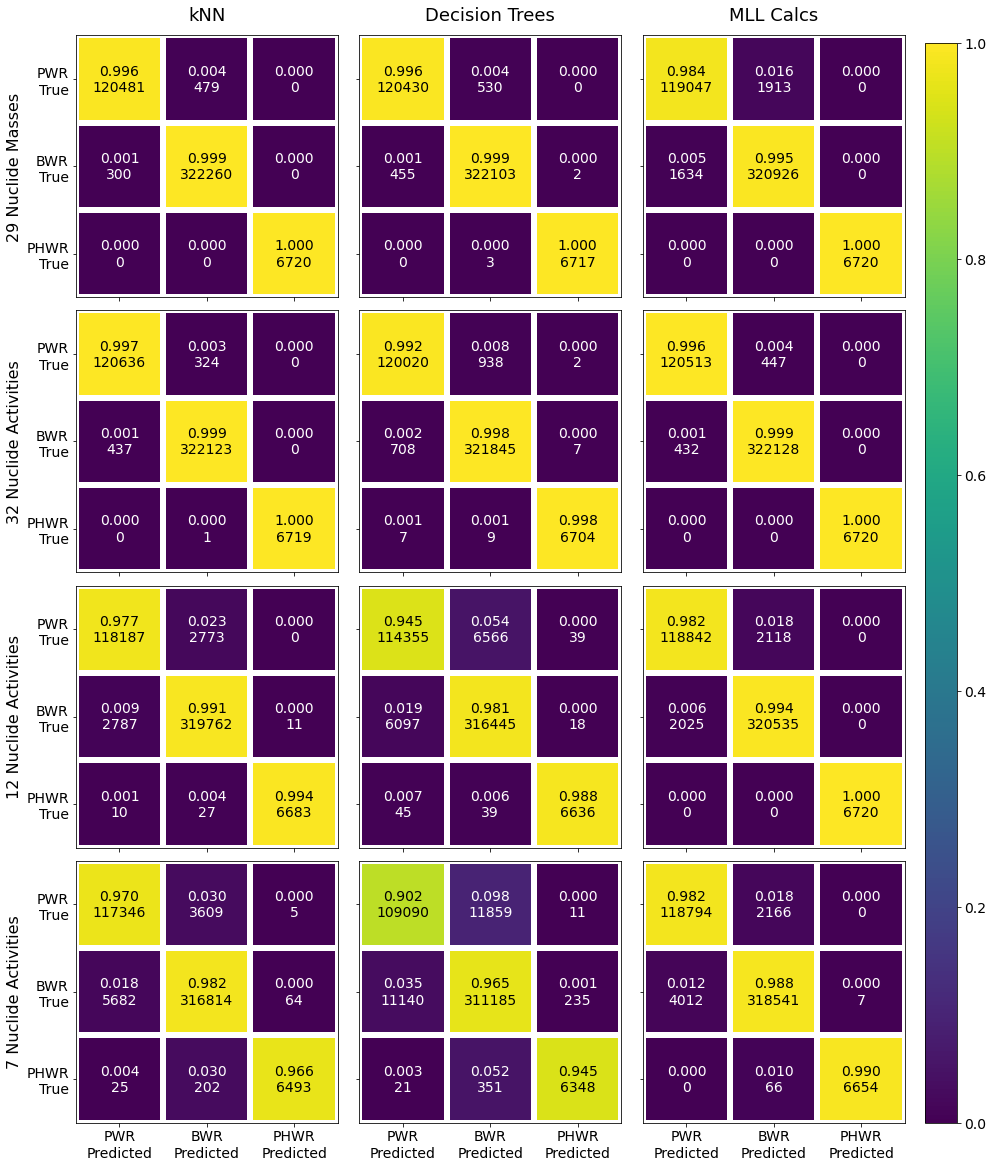
\includegraphics[width=\textwidth]{./chapters/exp2/confusion_matrix_nucs_acts.png}
  \caption{Confusion matrices of reactor type prediction for each algorithm 
           for different training sets (all at a 1\% error level): 29 nuclide 
           masses, 32 nuclide activities, 12 nuclide activities, and 7 nuclide 
           activities.}
  \label{fig:cm_nucs_acts}
\end{figure}

\begin{figure}[H]
  \centering
  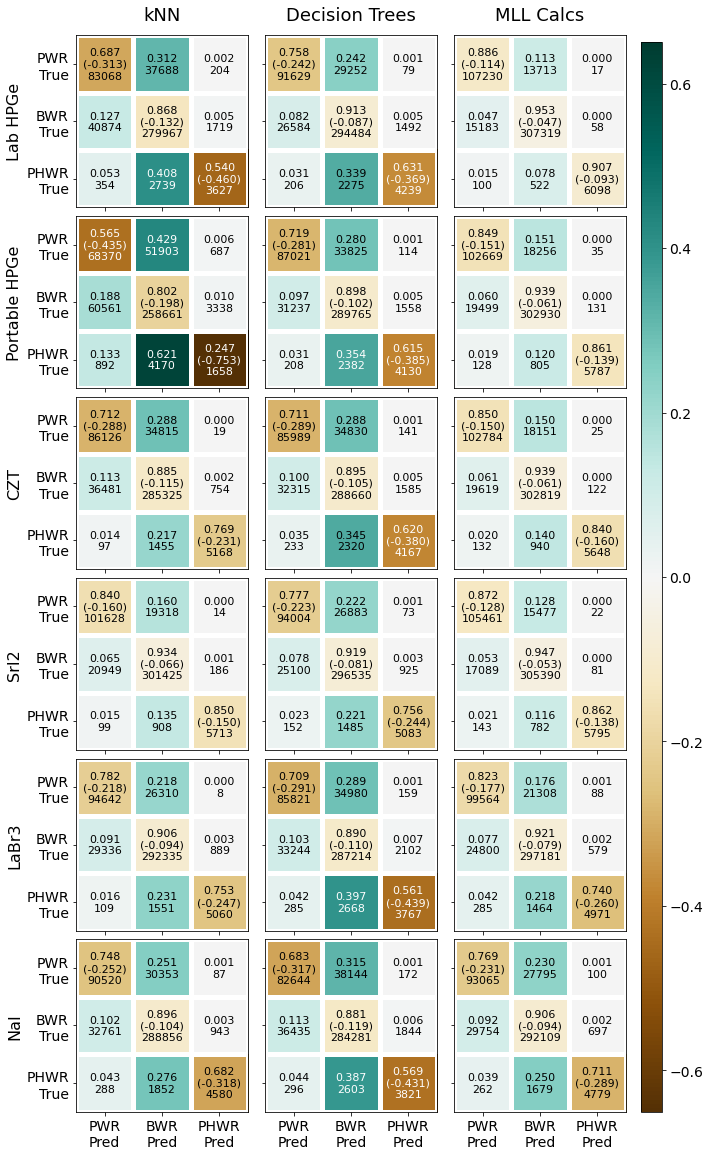
\includegraphics[width=0.83\textwidth]{./chapters/exp2/confusion_matrix_6dets_auto.png}
  \caption{Confusion matrices for auto energy window list training sets.}
  \label{fig:cm_auto}
\end{figure}

\begin{figure}[H]
  \centering
  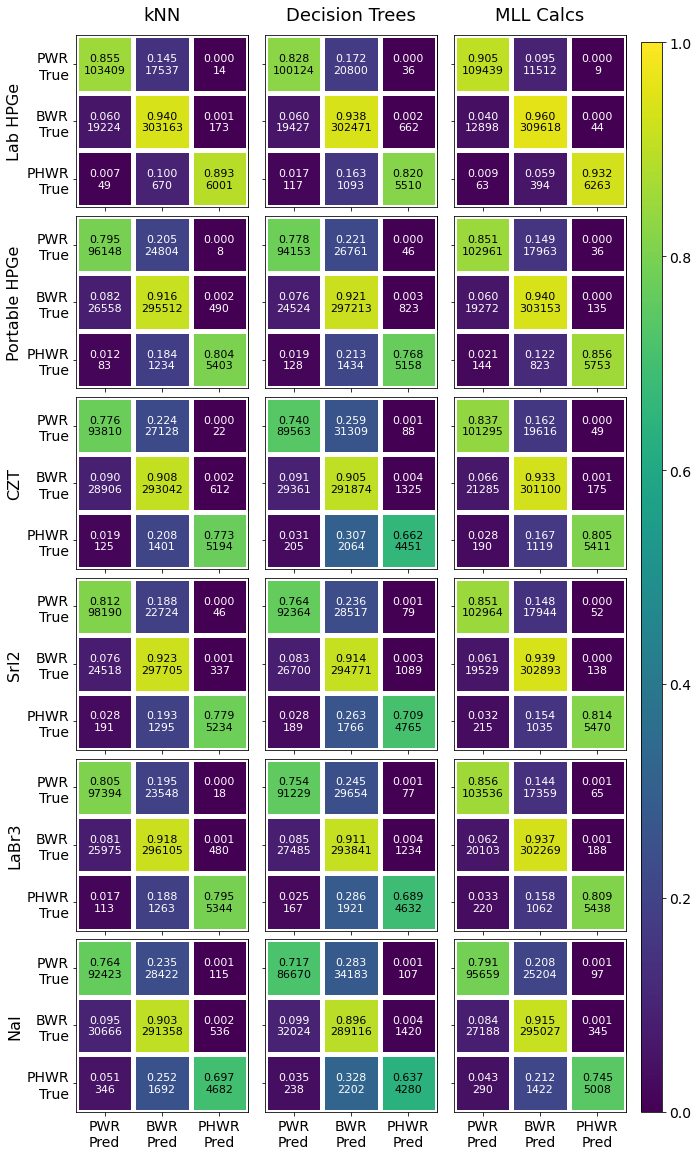
\includegraphics[width=0.83\textwidth]{./chapters/exp2/confusion_matrix_6dets_short.png}
  \caption{Confusion matrices for short energy window list training sets.}
  \label{fig:cm_short}
\end{figure}

\begin{figure}[H]
  \centering
  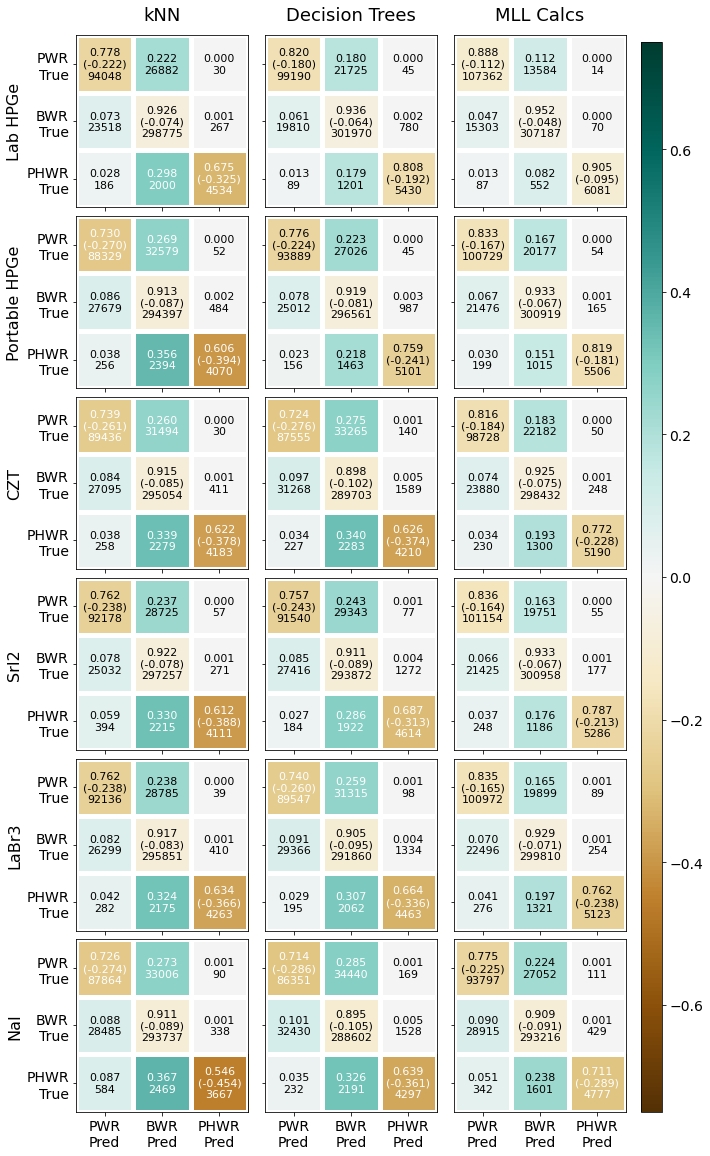
\includegraphics[width=0.83\textwidth]{./chapters/exp2/confusion_matrix_6dets_long.png}
  \caption{Confusion matrices for long energy window list training sets.}
  \label{fig:cm_long}
\end{figure}

Figure \ref{fig:cm_auto} shows the confusion matrices for all six detectors (in
the same order top-to-bottom as the \textit{x}-axis in Figure \ref{fig:rxtr})
for the auto energy windows list training sets. The \textit{k}-nearest
neighbors performances for the two \gls{HPGe}s were notably poor in the plot,
and the confusion matrices for these two cases explains why: not only are
40.8\% and 62.1\% of \gls{PHWR}s being misclassified as \gls{BWR}s for the
lab-based and portable \gls{HPGe}s, respectively, 31.2\% and 42.9\% of the
\gls{PWR}s are misclassified as \gls{BWR}s for the same two detectors,
respectively. By contrast, the second-best performing \textit{k}-nearest
neighbors-predicted detector case was the auto energy windows list for
\gls{SrI2}. The confusion matrix (in the fourth panel) for that data point 
shows 

\todo[inline]{come back to this: discussion incomplete. I think most of the
discussion will focus on PWR/PHWR being misclassified as BWR, since that is the
main two sources of misclassification.  The other squares stay pretty purple.}

